\chapter{\Kieker\ Analysis Component}
      % The analysis works a little bit different, that is why we explain it here.
      \KiekerAnalysis\ is the part of \Kieker\ which is responsible for the analysis, consisting of the reader, the consumer and the analysis instance itself. After we stored somewhere our records, we need to read them again somehow. This is task of the reader. Whatever we want to do with these informations is task of the consumers. They can for example evaluate, process or visualize the data. The analysis instance concerns about the lifetime and registration of the other parts.\\
      The analysis consists roughly of the following steps:
      \begin{enumerate}
	\item Create one (or more) analysis instance.
	\item Set the reader of this instance and line it with the necessary informations to read the stored records.
	\item Register the consumers who should do something with the recorded data.
	\item Start the analysis instance.
      \end{enumerate}
      % For the moment we don't have ANY configuration for the analysis part. This has to be done in the program.
      % \section{Configuration}

      \section{Readers}
	The \textit{monitoring log readers} (their position can be found in figure \ref{image:kiekercomponentdiagram}) are the direct counterpart to the \hyperlink{monitoringlogwriters}{\textit{monitoring log writers}}. While the writers get a record and write them in files or somewhere else, the readers take the writen data (from files, databases and so on) and convert them into a suitable instance of \textit{AbstractKiekerMonitoringRecord}. That means, that whenever we are implementing a new writer, we should also implement a corresponding reader. If we want for example save our recorded informations in a database, we have to be capable of reading these stored informations from the database again.\\
	Again there are some readers already implemented in \Kieker\ but we can implement an own reader as well. The following diagram shows the rough hierarchy.
	% This is the diagram with a simple reader hierarchy.
	\begin{figure}[H]
	  \begin{center}
	    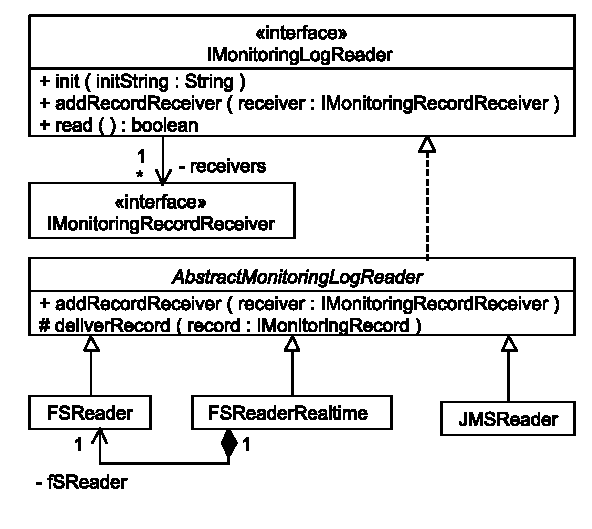
\includegraphics[width=0.5\textwidth]{./images/kieker_readerimpls.pdf}
	    \caption{The simple inheritance hierarchy of some currently implemented monitoring log readers}
	    \label{image:readers}
	  \end{center}
	\end{figure}
	The implementing of an own reader is nearly the same as the implementing of the writer, but to keep things simple, it is recommended to extend the already implemented AbstractKiekerMonitoringLogReader, because otherwise it would be necessary to implement the used observer pattern of the reader. By using the methods of the abstract class \textit{kieker.analysis.reader.AbstractMonitoringLogReader}, the task of delivering a new record to the consumers can be delegated to the super class.\\
	The following listing shows a simple reader which reads a stored record from the pipe. If there is nothing on the pipe to be read, the reader waits 4 seconds at maximum before it terminates.
	\setJavaCodeListing
	\lstset{caption=MyReader.java}
	\lstinputlisting{source-example/monitoring-and-analysis-with-own-components/src/mySimpleKiekerExample/bookstoreTracing/MyReader.java}

      \section{Consumers}
	The consumers are the parts of \Kieker\ which work with the records that have been loaded by the reader. There can be (theoretically) an infinite number of consumers which produce any kind of output. A consumer can be programmed by implementing the interface \textit{kieker.analysis.plugin.IMonitoringRecordConsumerPlugin} and implementing the necessary methods. Our following example consumer takes the given record and writes the content to the default output stream.
	\setJavaCodeListing
	\lstset{caption=MyConsumer.java}
	\lstinputlisting{source-example/monitoring-and-analysis-with-own-components/src/mySimpleKiekerExample/bookstoreTracing/MyConsumer.java}

      \section{The analysis}
	To put everything together, the following listing shows how to use the above-mentioned components.
	% It is not necessary to show the whole method.
	\setJavaCodeListing
	\begin{lstlisting}
	  AnalysisInstance ai = new AnalysisInstance();
	  MyReader reader = new MyReader();
	  reader.init("somePipe");
	  ai.setLogReader(reader);
	  ai.registerPlugin(new MyConsumer());
	  ai.run();
	\end{lstlisting}